\documentclass[10pt,journal,compsoc]{IEEEtran}

\usepackage{amsmath,amssymb,amsfonts}
\usepackage{algorithmic}
\usepackage{graphicx}
\usepackage{textcomp}
\usepackage{xcolor}
\usepackage{booktabs}
\usepackage{multirow}
\usepackage{url}
\usepackage{cite}
\usepackage{hyperref}
\usepackage{cleveref}
\usepackage{microtype}

\hypersetup{
    colorlinks=true,
    linkcolor=blue,
    filecolor=magenta,      
    urlcolor=cyan,
    citecolor=blue,
}

\begin{document}

\title{Multimodal Time Series Models: A Survey and Outlook}

\author{Huirui~Li
\thanks{H. Li is with the School of Computer Science. Project repository and continuous review updates: \url{https://github.com/lihuirui/awesome-multimodal-time-series-survey}. Correspondence: 58367737+lihuirui@users.noreply.github.com.}
}

\markboth{IEEE Transactions on Pattern Analysis and Machine Intelligence (Preprint), Vol.~14, No.~8, September~2026}%
{Li: Multimodal Time Series Models: A Survey and Outlook}

\IEEEtitleabstractindextext{%
\begin{abstract}
Time series analysis is foundational to critical cyber-physical and natural systems, spanning climate science, financial forecasting, clinical health monitoring, smart grids, and intelligent transportation. While traditional paradigms and unimodal deep learning models rely exclusively on discrete numerical records, real-world systems are embedded in rich multimodal contexts—accompanied by news reports, natural language operational logs, visual charts, and spatial topologies. Recently, the confluence of Large Language Models (LLMs), Vision-Language Models (VLMs), and pre-trained Time Series Foundation Models (TSFMs) has catalyzed a paradigm shift toward Multimodal Time Series Models. This survey provides the first comprehensive, systematic review (following PRISMA 2020 guidelines) of multimodal time series research from 2021 to 2026. We formalize the multimodal time series problem, propose a multi-dimensional taxonomy decomposing the literature by modality pairing, fusion architecture, the functional role of complementary modalities, and downstream tasks. Furthermore, we categorize cutting-edge methodologies including cross-modal patch reprogramming, visual line-chart transcoding, unified multimodal tokenization, and neuro-symbolic reasoning agents. We benchmark the evolving dataset landscape, scrutinize persistent challenges—including cross-modal distribution gaps, temporal misalignment, and evaluation leakage—and outline high-leverage future research directions.
\end{abstract}

\begin{IEEEkeywords}
Multimodal Learning, Time Series Analysis, Large Language Models, Vision-Language Models, Foundation Models, Temporal Reasoning.
\end{IEEEkeywords}}

\maketitle
\IEEEdisplaynontitleabstractindextext
\IEEEpeerreviewmaketitle

\section{Introduction}
\label{sec:intro}

Time series data represents the temporal pulse of our interconnected physical, biological, and socio-economic systems. Over the past several decades, the study of temporal sequence modeling has evolved across three major technological waves: classical statistical and autoregressive modeling (e.g., ARIMA, exponential smoothing), task-specific deep neural architectures (e.g., RNNs, LSTMs, TCNs, Informer, PatchTST), and most recently, large pre-trained Time Series Foundation Models (TSFMs)~\cite{Goswami2024MOMENT,Liu2024Timer,Ansari2024Chronos,Ekambaram2024TTM}. 

Despite extraordinary advances in univariate and multivariate numerical modeling, an essential constraint persists across unimodal paradigms: \textit{real-world temporal dynamics do not unfold in an informational vacuum}. When a sudden traffic congestion spike occurs, an electrical grid frequency deviates, or a stock price undergoes rapid volatility, the underlying generative causes are rarely confined to historical numerical values alone. Instead, these phenomena are profoundly shaped by external multimodal signals: breaking news reports, meteorological alerts, natural language operational dispatches, visual monitoring streams, and relational graph topologies. 

\begin{figure*}[t]
\centering
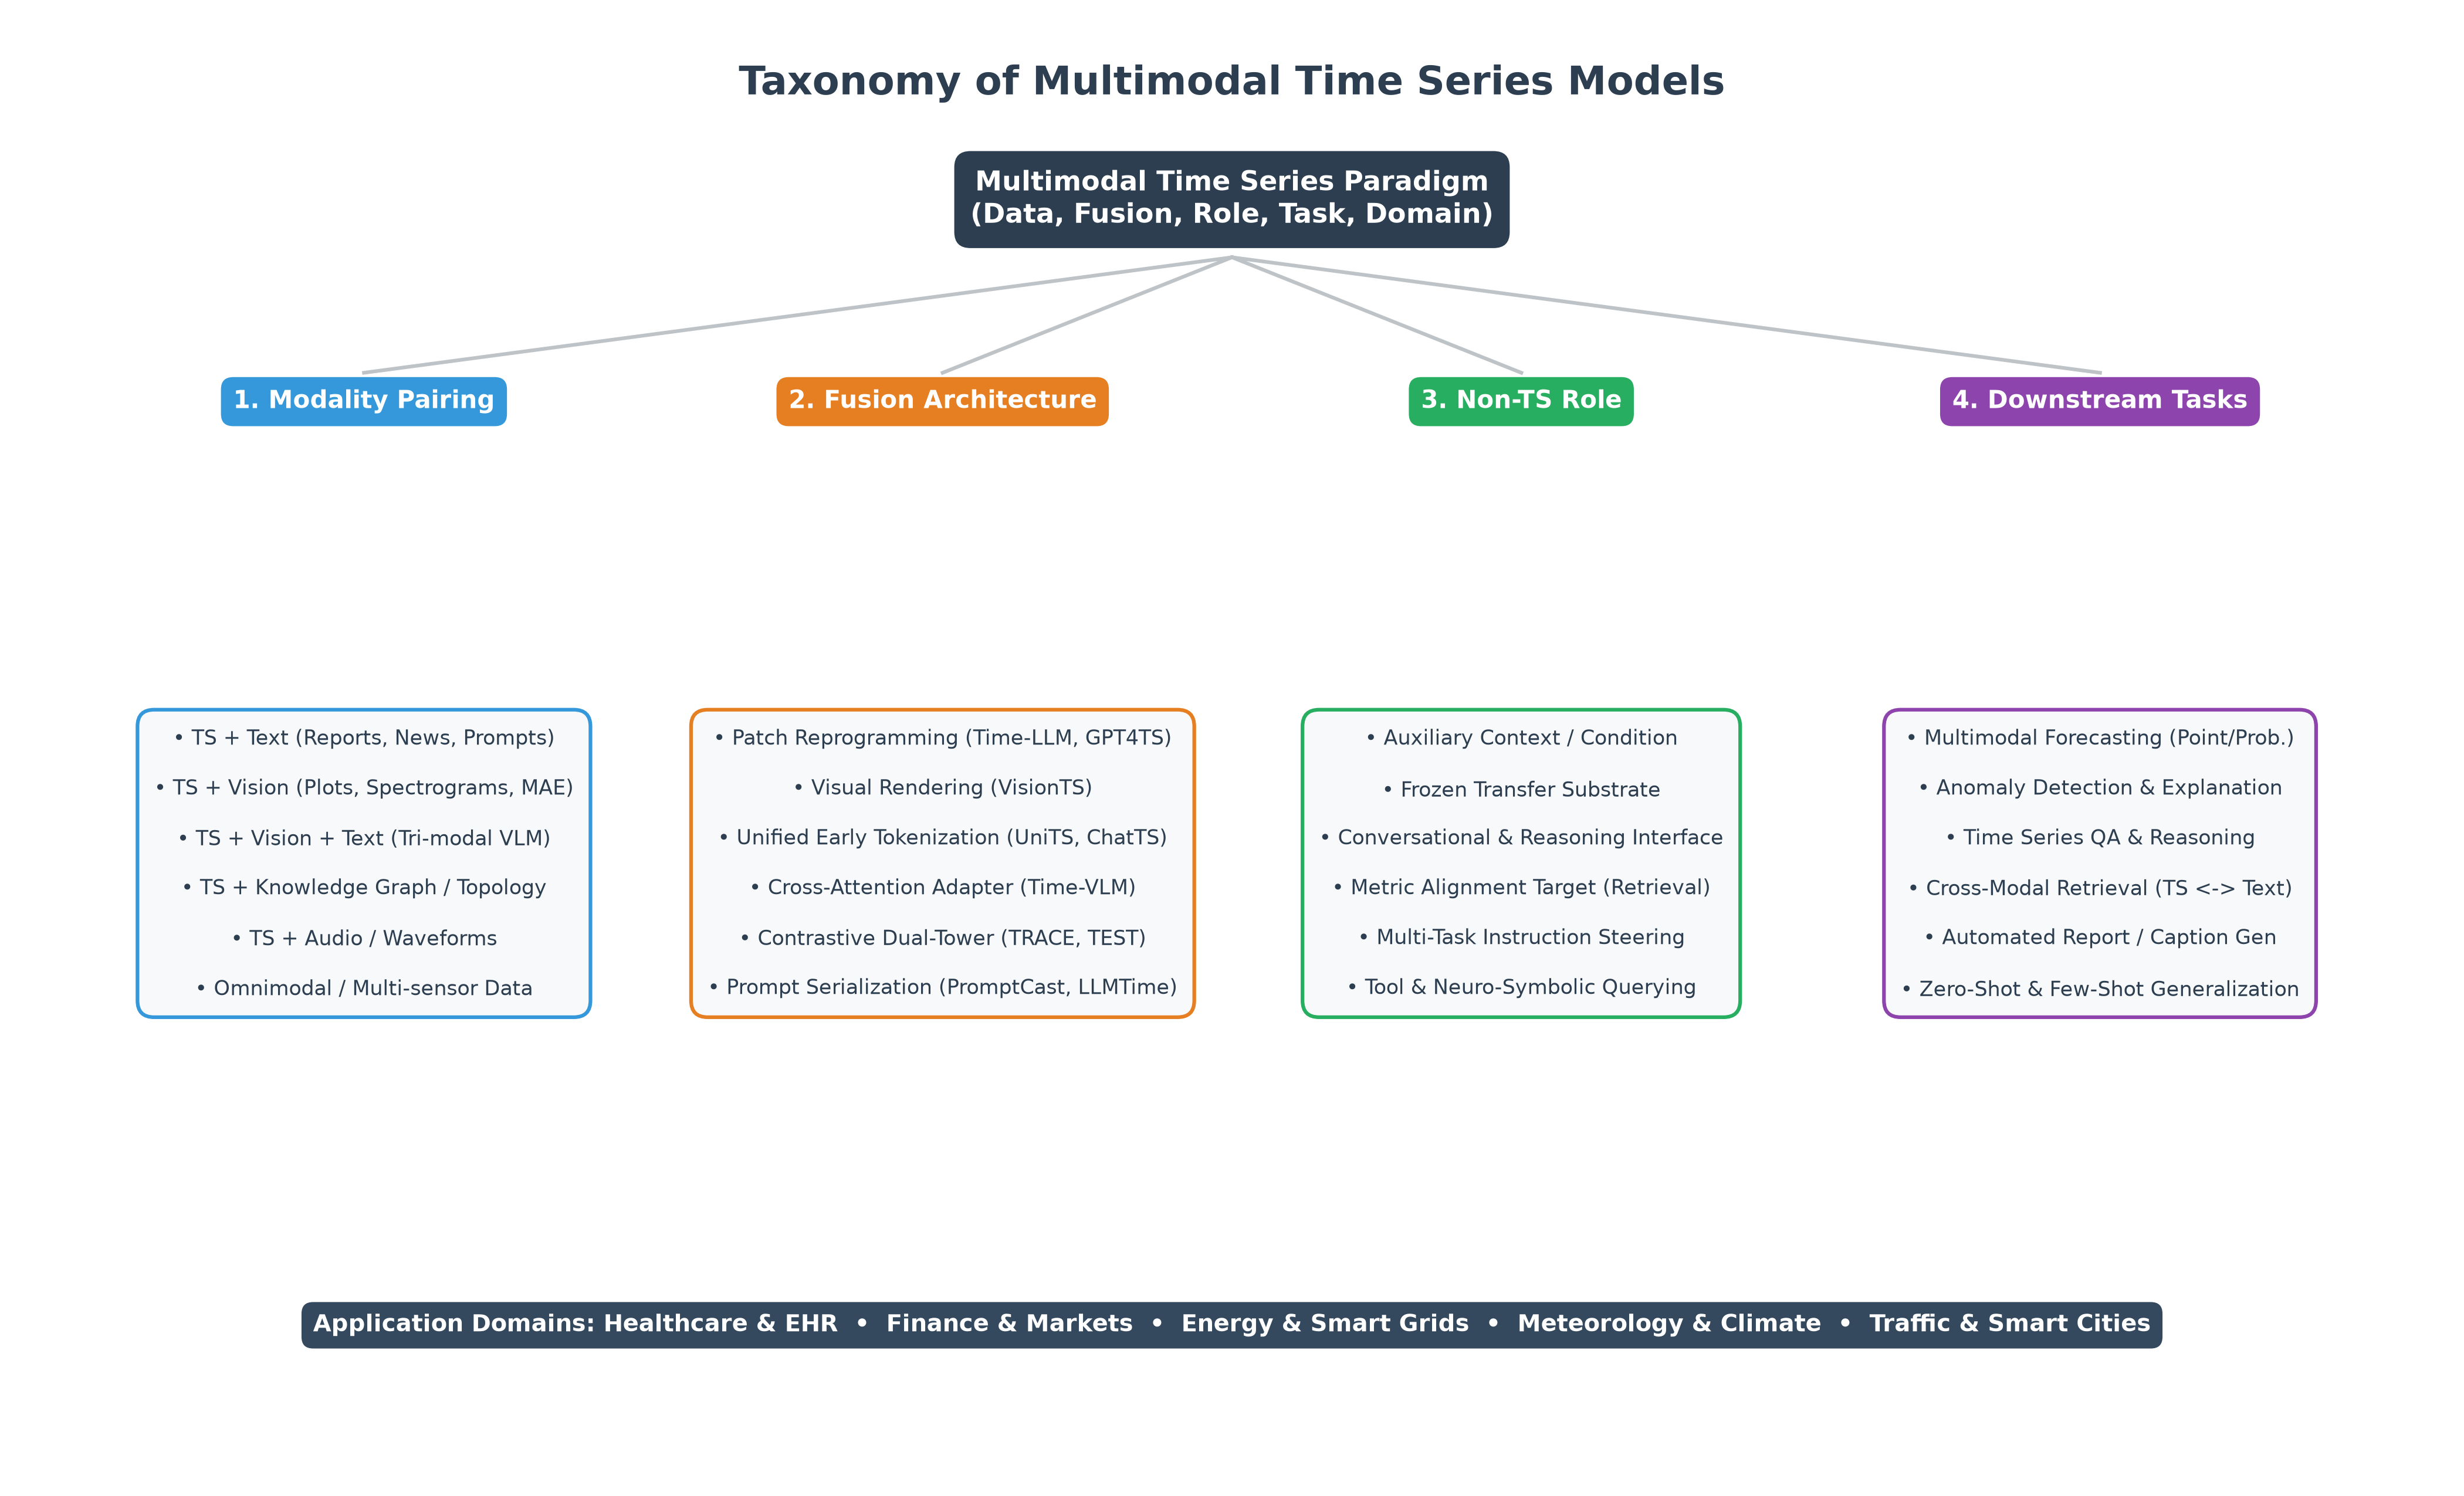
\includegraphics[width=0.98\textwidth]{figures/taxonomy.png}
\caption{The proposed multidimensional taxonomy for multimodal time series models, organizing the literature across four core pillars: Modality Pairing, Fusion Architecture, Role of the Complementary Modality, and Downstream Predictive/Analytical Tasks across diverse application domains.}
\label{fig:taxonomy}
\end{figure*}

\subsection{The Rise of Multimodal Time Series Intelligence}
The unprecedented general reasoning capabilities of pre-trained Large Language Models (LLMs) and Vision-Language Models (VLMs) have fundamentally transformed artificial intelligence. Researchers quickly observed that the sequence modeling principles governing language and vision exhibit deep mathematical parallels with time series. This has catalyzed an explosion of research exploring the intersection of time series and multimodal models:
\begin{enumerate}
    \item \textbf{Cross-Modal Reprogramming:} Groundbreaking frameworks such as Time-LLM~\cite{Jin2023TimeLLM} and One Fits All (GPT4TS)~\cite{Zhou2023OneFitsAll} demonstrated that frozen language model backbones (e.g., GPT-2, LLaMA) can be repurposed as high-accuracy time-series forecasters by patching time series and aligning temporal representations with textual semantic prompts.
    \item \textbf{Visual Transcoding \& Vision-Language Synergy:} Counter-intuitively, VisionTS~\cite{Chen2024VisionTS} revealed that reformulating numeric series as line-chart images allows off-the-shelf visual masked autoencoders (MAE pre-trained on ImageNet) to perform competitive zero-shot forecasting without any domain fine-tuning. Concurrently, Time-VLM~\cite{Zhong2025TimeVLM} unites visual, textual, and temporal representations for augmented forecasting.
    \item \textbf{Conversational Reasoning \& TS-MLLMs:} Pioneering systems such as ChatTS~\cite{Zhao2024ChatTS}, TimeOmni-1~\cite{Tan2025TimeOmni1}, and ChatTime~\cite{ChatTime2024} elevate time-series models from passive function approximators to interactive reasoning agents capable of answering temporal questions, conducting counterfactual reasoning, and explaining anomalies.
    \item \textbf{Multimodal Datasets \& Benchmarks:} Systematic benchmarks such as Time-MMD~\cite{Liu2024TimeMMD}, Fidel-TS~\cite{FidelTS2025}, and MTBench~\cite{MTBench2025} have begun curating high-fidelity, aligned cross-modal time series corpora across diverse real-world domains.
\end{enumerate}

\begin{table*}[t]
\caption{Comparison of This Survey with Existing Surveys in Time Series and Large Models.}
\label{tab:survey_comparison}
\centering
\small
\resizebox{\textwidth}{!}{%
\begin{tabular}{lcccccc}
\toprule
\textbf{Survey Reference} & \textbf{Year} & \textbf{Scope Focus} & \textbf{TS Modalities} & \textbf{Cross-Modal Fusion} & \textbf{TS-MLLM Reasoning} & \textbf{PRISMA Protocol} \\
\midrule
Jin et al.~\cite{Jin2023LargeModelsSurvey} & 2023 & Large Models (TS \& ST) & TS + Spatio-Temporal & Partial & Limited & No \\
Jin et al.~\cite{Jin2024PositionLLMTS} & 2024 & Position: LLMs for TS & Numerical TS & Reprogramming focus & Preliminary & No \\
\textbf{This Survey} & \textbf{2026} & \textbf{Multimodal TS Models} & \textbf{TS + Text + Vision + KG} & \textbf{Comprehensive} & \textbf{In-Depth (2021--2026)} & \textbf{Yes (PRISMA 2020)} \\
\bottomrule
\end{tabular}%
}
\end{table*}

\subsection{Need for a Dedicated Survey}
While prior comprehensive surveys have examined large foundation models for pure time-series or spatio-temporal data~\cite{Jin2023LargeModelsSurvey,Jin2024PositionLLMTS}, they predominantly focus on unimodal foundation architectures or single-modality adaptation. As shown in \Cref{tab:survey_comparison}, there lacks a dedicated, systematic survey synthesizing the rapid evolution of \textit{explicitly multimodal time series modeling}—spanning text-guided forecasting, vision-based time series modeling, multi-task unified architectures, and conversational reasoning agents.

\subsection{Contributions of This Survey}
To fill this critical void, this paper provides:
\begin{itemize}
    \item \textbf{A Systematic, Verifiable Review:} Conducted under the PRISMA 2020 framework spanning 2021 to 2026, where every cited paper is verified against authoritative bibliographic APIs.
    \item \textbf{A Four-Pillar Taxonomy:} A taxonomy deconstructing multimodal time series research along Modality Pairing, Fusion Architecture, Non-TS Role, and Downstream Tasks (\Cref{fig:taxonomy}).
    \item \textbf{Deep Methodological Analysis:} A unified comparative dissection of cross-modal reprogramming, visual line-chart transcoding, contrastive alignment, and interactive reasoning architectures.
    \item \textbf{Curated Resource \& Dataset Landscape:} An exhaustive mapping of multimodal benchmark datasets, open-source repositories, and evaluation protocols.
    \item \textbf{Critical Perspectives on Open Challenges:} A rigorous appraisal of the modality gap, benchmark data contamination, temporal granularity mismatches, and future research trajectories.
\end{itemize}

\section{Background \& Preliminaries}
\label{sec:background}

In this section, we formally formulate the multimodal time-series modeling problem, detail the standard mathematical representations of temporal and non-temporal modalities, and review foundational learning objectives.

\subsection{Problem Formulation}

\textbf{Definition 1 (Multivariate Time Series).} Let $\mathbf{X}_{1:T} = [\mathbf{x}_1, \mathbf{x}_2, \dots, \mathbf{x}_T]^\top \in \mathbb{R}^{T \times C}$ denote a continuous or discrete multivariate temporal sequence observed over $T$ uniform time steps across $C$ feature channels, where $\mathbf{x}_t = [x_{t,1}, x_{t,2}, \dots, x_{t,C}]^\top \in \mathbb{R}^C$.

\textbf{Definition 2 (Complementary Multimodal Context).} In a multimodal setting, the time series $\mathbf{X}_{1:T}$ is paired with complementary non-temporal contextual information $\mathcal{M} = \{\mathbf{M}_{\text{text}}, \mathbf{M}_{\text{vis}}, \mathbf{M}_{\text{graph}}\}$, where:
\begin{itemize}
    \item $\mathbf{M}_{\text{text}} = (w_1, w_2, \dots, w_L)$ represents a sequence of discrete linguistic tokens (e.g., domain descriptions, incident logs, financial news, or analytical instructions).
    \item $\mathbf{M}_{\text{vis}} \in \mathbb{R}^{H \times W \times 3}$ denotes a 2D visual representation (e.g., plotted line charts, spectrogram transforms, or synchronous satellite imagery).
    \item $\mathbf{M}_{\text{graph}} = (\mathcal{V}, \mathcal{E}, \mathbf{A})$ encapsulates topological or spatial relationships connecting multivariate time-series nodes.
\end{itemize}

\textbf{Definition 3 (Multimodal Time Series Objective).} Given an observed history $\mathbf{X}_{1:T}$ and context $\mathcal{M}$, the goal is to parameterize a model $f_\Theta$ that maps $\{\mathbf{X}_{1:T}, \mathcal{M}\}$ to a target space $\mathbf{Y}$ (which may represent future horizons $\mathbf{X}_{T+1:T+H}$, anomaly labels $\mathbf{y} \in \{0, 1\}^T$, textual answers, or joint embeddings) by minimizing an expected loss:
\begin{equation}
\min_\Theta \mathbb{E}_{(\mathbf{X}, \mathcal{M}, \mathbf{Y})} \left[ \mathcal{L}_{\text{task}}(f_\Theta(\mathbf{X}_{1:T}, \mathcal{M}), \mathbf{Y}) + \lambda \mathcal{L}_{\text{align}}(\mathbf{X}_{1:T}, \mathcal{M}) \right]
\label{eq:general_loss}
\end{equation}
where $\mathcal{L}_{\text{align}}$ denotes cross-modal alignment regularization.

\subsection{Temporal Patching and Tokenization}
Direct point-wise numerical tokenization often suffers from high computational overhead and lacks semantic density. Following modern practice~\cite{Zhou2023OneFitsAll,Jin2023TimeLLM}, continuous time series are transformed into $N$ temporal patches of length $P$ with stride $S$:
\begin{equation}
\mathbf{P}_i = \mathbf{x}_{(i-1)S : (i-1)S + P} \in \mathbb{R}^{P \times C}, \quad i \in \left\{1, \dots, N = \left\lfloor \frac{T - P}{S} \right\rfloor + 1 \right\}
\end{equation}
Each patch $\mathbf{P}_i$ is linearly projected into a $d_{\text{model}}$-dimensional continuous latent embedding and augmented with learnable temporal position encoding $\mathbf{E}_{\text{pos}}$:
\begin{equation}
\mathbf{h}_i = \mathbf{P}_i \mathbf{W}_{\text{in}} + \mathbf{E}_{\text{pos}, i}, \quad \mathbf{W}_{\text{in}} \in \mathbb{R}^{(P \cdot C) \times d_{\text{model}}}
\label{eq:patch_projection}
\end{equation}

\subsection{Cross-Modal Alignment Paradigms}
Multimodal architectures leverage three primary pre-training and alignment paradigms:
\begin{enumerate}
    \item \textbf{Contrastive Representation Learning (InfoNCE):} Given paired time series representations $\mathbf{z}^{\text{ts}}$ and context representations $\mathbf{z}^{\text{text}}$, a dual-encoder minimizes the normalized temperature-scaled cross-entropy~\cite{Sun2023TEST,Chen2025TRACE}:
    \begin{equation}
    \mathcal{L}_{\text{InfoNCE}} = -\log \frac{\exp(\text{sim}(\mathbf{z}_i^{\text{ts}}, \mathbf{z}_i^{\text{text}}) / \tau)}{\sum_{j=1}^B \exp(\text{sim}(\mathbf{z}_i^{\text{ts}}, \mathbf{z}_j^{\text{text}}) / \tau)}
    \label{eq:infonce}
    \end{equation}
    \item \textbf{Masked Autoencoding (MAE):} In visual or temporal reconstruction, a subset of patches $\mathcal{M}_{\text{mask}} \subset \{1, \dots, N\}$ is masked out, and the model reconstructs the unobserved temporal values from visible tokens~\cite{Chen2024VisionTS}:
    \begin{equation}
    \mathcal{L}_{\text{MAE}} = \frac{1}{|\mathcal{M}_{\text{mask}}|} \sum_{i \in \mathcal{M}_{\text{mask}}} \|\mathbf{P}_i - \hat{\mathbf{P}}_i\|_2^2
    \end{equation}
    \item \textbf{Autoregressive Next-Token Prediction:} In decoder-only LLM-adapted forecasters, predictions are generated sequentially conditioned on prefix prompt tokens $\mathbf{E}_{\text{prompt}}$ and temporal patch tokens~\cite{Liu2024AutoTimes,Zhao2024ChatTS}:
    \begin{equation}
    \mathcal{L}_{\text{AR}} = -\sum_{t=1}^K \log P(y_t \mid y_{<t}, \mathbf{E}_{\text{prompt}}, \mathbf{h}_{1:N})
    \end{equation}
\end{enumerate}

\section{Taxonomy of Multimodal Time Series Models}
\label{sec:taxonomy}

To provide a rigorous structural foundation for this survey, we propose a multi-dimensional taxonomy deconstructing the literature across four orthogonal pillars: (1)~\textbf{Modality Pairing}, (2)~\textbf{Fusion Architecture}, (3)~\textbf{Functional Role of the Complementary Modality}, and (4)~\textbf{Downstream Tasks and Domains} (illustrated in \Cref{fig:taxonomy}).

\begin{figure*}[t]
\centering
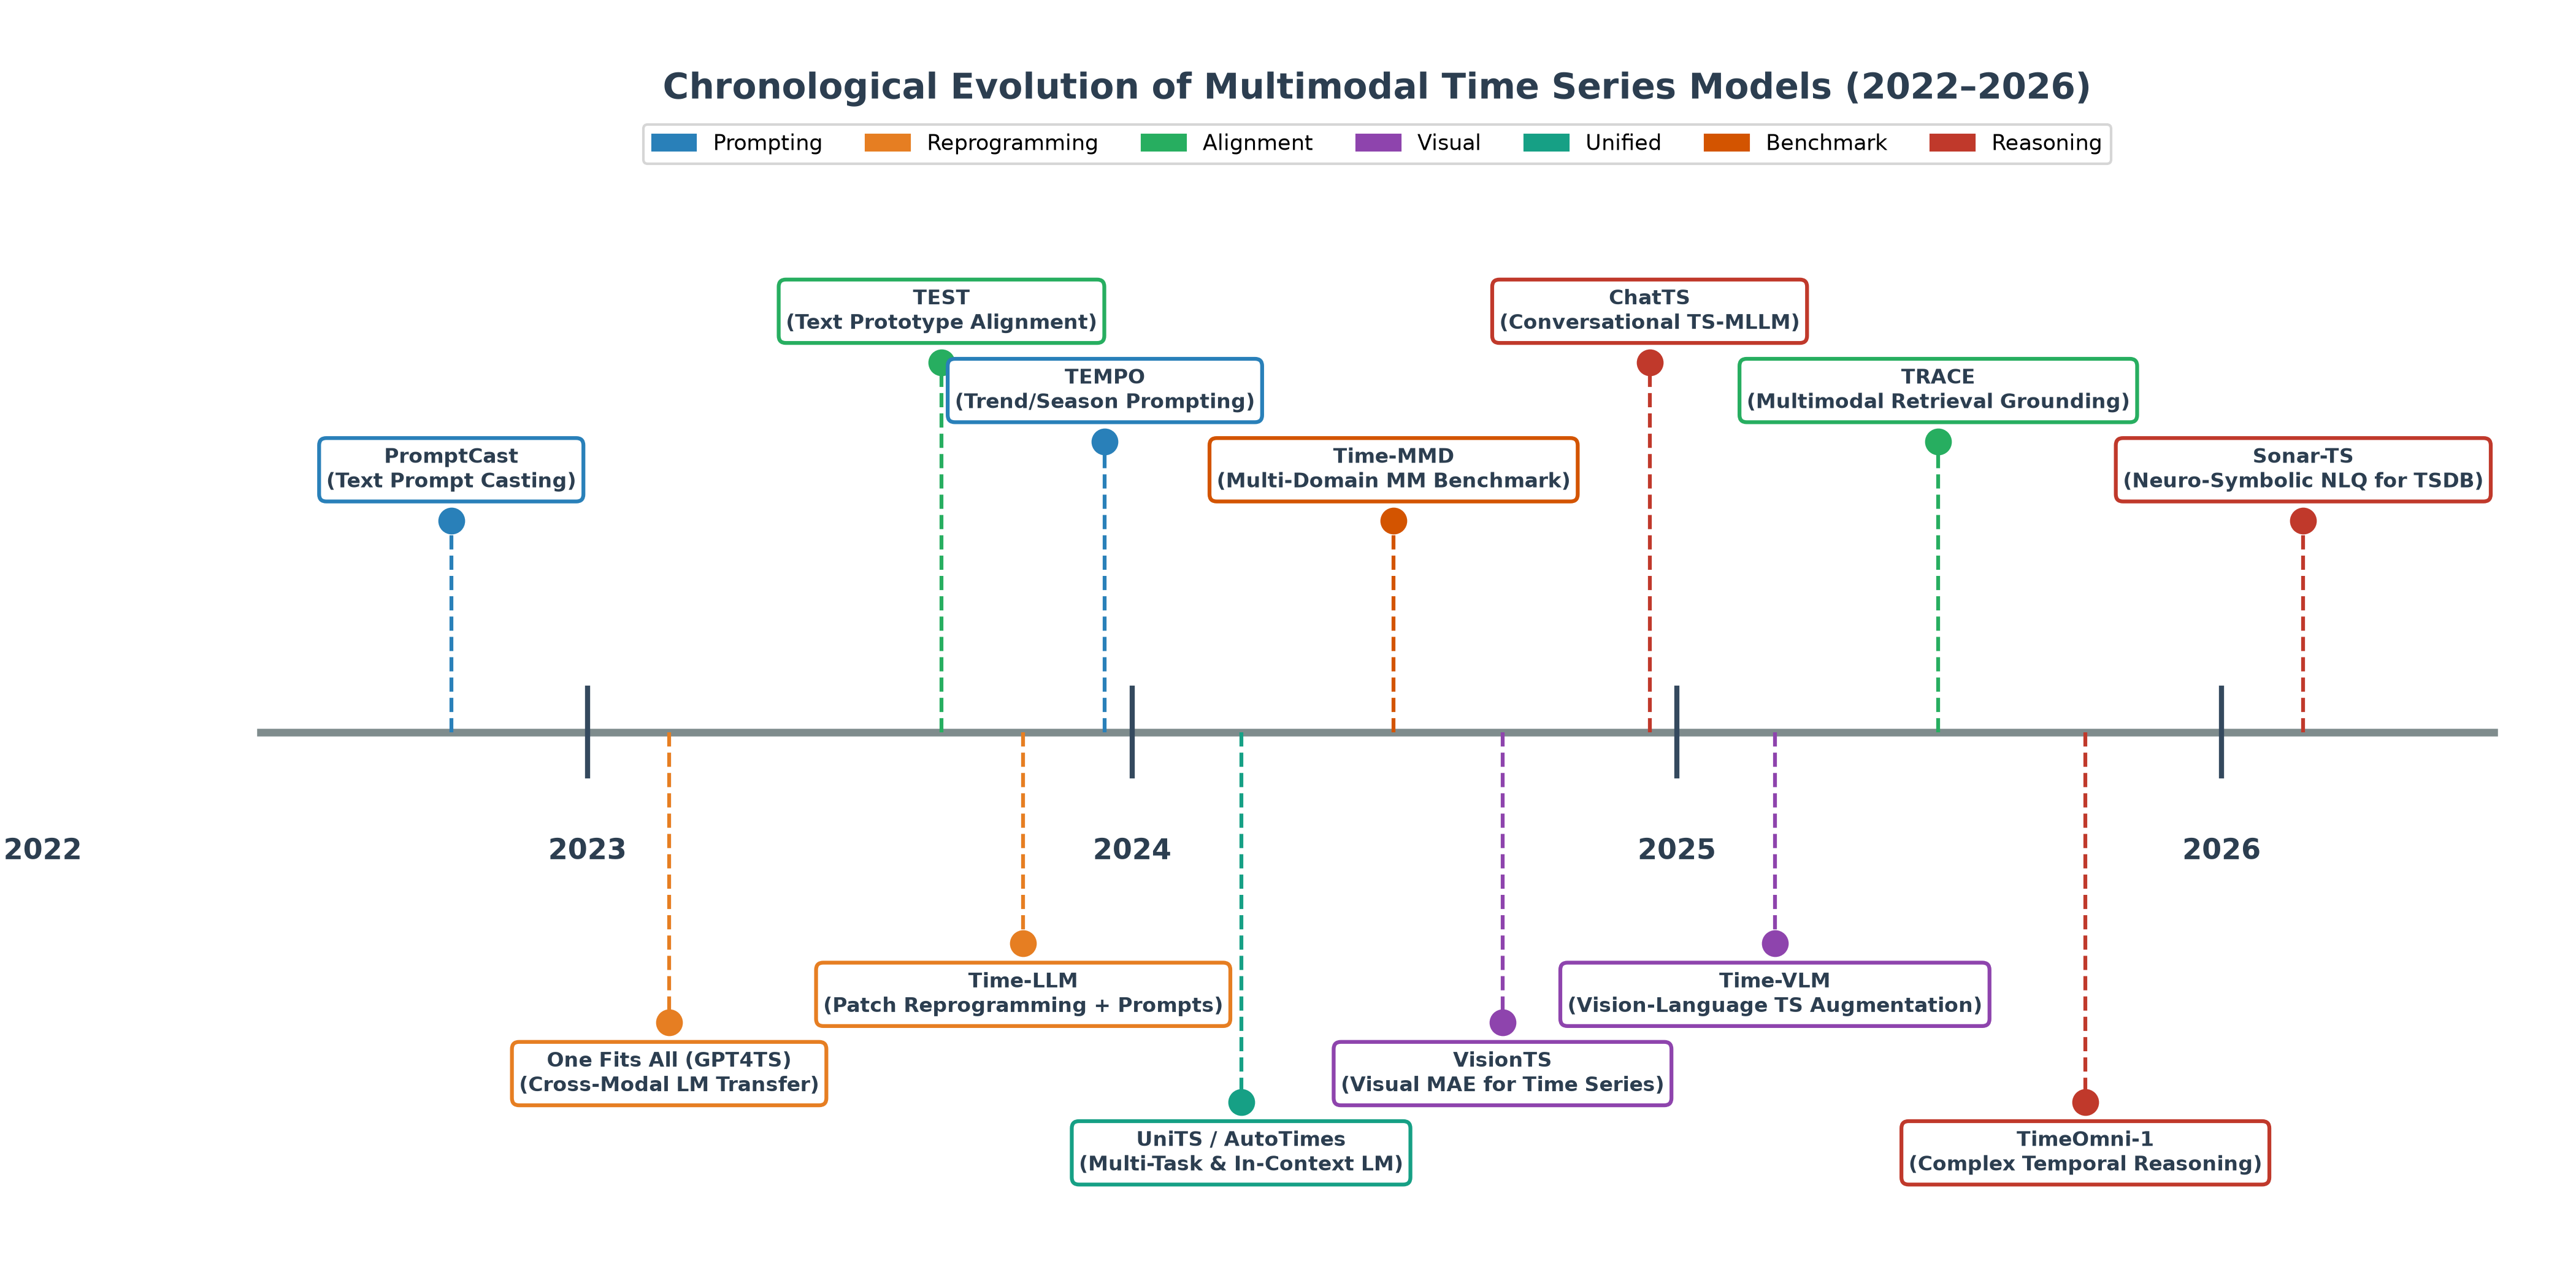
\includegraphics[width=0.98\textwidth]{figures/timeline_milestones.png}
\caption{Chronological milestones in multimodal time-series modeling from 2022 to 2026, illustrating the evolution from early text prompt casting (PromptCast) to cross-modal reprogramming (One Fits All, Time-LLM), visual transcoding (VisionTS), unified multimodal models (UniTS, Time-MMD), and neuro-symbolic reasoning frameworks (ChatTS, TimeOmni, Sonar-TS).}
\label{fig:timeline}
\end{figure*}

\subsection{Pillar 1: Modality Pairing}
The combinations of data modalities co-occurring with time series fundamentally dictate architectural constraints and inductive biases:
\begin{itemize}
    \item \textbf{Time Series + Text ($\text{TS} + \text{Text}$):} The most prominent paradigm. Text serves diverse functions: semantic descriptions (e.g., sensor metadata, sampling rates, geographical origins in Time-LLM~\cite{Jin2023TimeLLM} and TEMPO~\cite{Cao2023TEMPO}), continuous narrative reports (financial news, corporate filings, EHR medical notes in Time-MMD~\cite{Liu2024TimeMMD}), or natural language analytical queries~\cite{Zhao2024ChatTS,Xue2022PromptCast,Shen2025TimeMQA}.
    \item \textbf{Time Series + Vision ($\text{TS} + \text{Vision}$):} Exploits 2D visual representations—either by directly plotting numerical trajectories as line charts (VisionTS~\cite{Chen2024VisionTS}, VisionTS++~\cite{Chen2025VisionTSPlus}) or converting temporal signals into 2D spectrograms—to harness vision foundation models pre-trained on massive natural image corpora without manual task redesign.
    \item \textbf{Time Series + Audio / Acoustic Waveforms ($\text{TS} + \text{Audio}$):} Exemplified by Voice2Series~\cite{Yang2021Voice2Series} and SeisT~\cite{Zhang2024SeisT}. Continuous 1D acoustic and seismic waveforms share strong mathematical analogies with time series (e.g., frequency harmonics, non-stationary oscillatory wavelets), enabling cross-domain reprogramming from pre-trained speech/audio models.
    \item \textbf{Time Series + Spatio-Temporal Physical Grids ($\text{TS} + \text{Grid}$):} Foundational in Earth systems science (ClimaX~\cite{Nguyen2023ClimaX}, Prithvi WxC~\cite{Schmude2024PrithviWxC}, Aurora~\cite{Bodnar2024Aurora}). Here, multivariate temporal sequences are coupled with multi-level geospatial grids governed by atmospheric thermodynamics and fluid dynamics equations.
    \item \textbf{Time Series + Clinical Imaging ($\text{TS} + \text{Clinical}$):} MedFuse~\cite{Hayat2022MedFuse} couples irregularly sampled physiological ICU signals with paired chest X-rays, reconciling high-frequency temporal trajectories with static diagnostic scans.
    \item \textbf{Tri-Modal \& Omnimodal Systems ($\text{TS} + \text{Vision} + \text{Text}$):} Recent unified architectures, notably Time-VLM~\cite{Zhong2025TimeVLM} and TimeOmni-1~\cite{Tan2025TimeOmni1}, combine temporal sequences with synchronized visual views and textual context for holistic multi-sensory understanding.
\end{itemize}

\subsection{Pillar 2: Fusion Architecture}
How representations from disparate modalities are mathematically merged constitutes the core engineering challenge:
\begin{enumerate}
    \item \textbf{Cross-Modal Patch Reprogramming:} Keeps the backbone foundation model (e.g., LLaMA, GPT-2, acoustic nets) completely frozen. Patch-level linear or multi-head attention projection layers reprogram numerical time-series patches into the continuous embedding space of language or acoustic tokens~\cite{Yang2021Voice2Series,Jin2023TimeLLM,Zhou2023OneFitsAll,Chang2023LLM4TS,Liu2024CALF}.
    \item \textbf{Modality Transcoding \& Continual Vision Adaptation:} Transforms the temporal sequence into another modality prior to ingestion. VisionTS~\cite{Chen2024VisionTS} and VisionTS++~\cite{Chen2025VisionTSPlus} render normalized time series into pixel bitmaps, bypassing numerical tokenization entirely and processing the visual stream with ViT-based Masked Autoencoders.
    \item \textbf{Variable-Tokenized Physics Transformers:} Introduced by ClimaX~\cite{Nguyen2023ClimaX} and scaled by Prithvi WxC~\cite{Schmude2024PrithviWxC} and Aurora~\cite{Bodnar2024Aurora}. Heterogeneous physical variables are tokenized independently with variable-specific projection weights, enabling arbitrary subsets of variables, lead times, and spatial resolutions to be processed uniformly.
    \item \textbf{Decoupled Alignment \& Language Masking:} UniTime~\cite{Liu2024UniTime} and TimeCMA~\cite{Liu2024TimeCMA} employ language-masked cross-attention and cross-modal feature calibration, dynamically guiding temporal feature extraction without entangling raw time-series representations.
    \item \textbf{Unified Early Tokenization:} Maps heterogeneous modalities into a shared token dictionary. Models such as UniTS~\cite{Gao2024UniTS} and ChatTime~\cite{ChatTime2024} tokenize time-series patches, instruction prompts, and domain markers into unified token embeddings passed jointly into deep Transformer stacks.
    \item \textbf{Dual-Tower Metric Alignment:} Maintains separate, dedicated encoders for time-series and textual context, aligning them in a shared latent metric space using contrastive losses (e.g., TRACE~\cite{Chen2025TRACE} and TEST~\cite{Sun2023TEST}).
\end{enumerate}

\subsection{Pillar 3: Functional Role of the Complementary Modality}
Rather than treating all modalities symmetrically, the complementary modality plays specific functional roles:
\begin{itemize}
    \item \textbf{Auxiliary Context / Inductive Condition:} Text or metadata acts as conditioning information to resolve ambiguity in numerical time series, mitigating non-stationarity (e.g., Time-LLM, TEMPO, $\text{S}^2\text{IP-LLM}$~\cite{Pan2024S2IPLLM}, UniTime~\cite{Liu2024UniTime}).
    \item \textbf{Frozen Transfer Substrate:} The language or acoustic model acts as an overparameterized pattern-matching backbone whose self-attention mechanisms transfer directly to universal time-series forecasting (One Fits All~\cite{Zhou2023OneFitsAll}, Voice2Series~\cite{Yang2021Voice2Series}).
    \item \textbf{Physics / Geophysical Invariance Prior:} Multi-level atmospheric grids enforce physical continuity and conservation laws (ClimaX~\cite{Nguyen2023ClimaX}, Aurora~\cite{Bodnar2024Aurora}).
    \item \textbf{Conversational \& Reasoning Interface:} The non-TS modality serves as an interactive communication interface, enabling open-ended question answering, root-cause diagnostics, and counterfactual simulation (ChatTS~\cite{Zhao2024ChatTS}, TimeOmni-1~\cite{Tan2025TimeOmni1}, Time-MQA~\cite{Shen2025TimeMQA}).
    \item \textbf{Retrieval Anchor:} Text serves as a semantic query anchor for indexing, clustering, and retrieving dynamic time-series trajectories (TRACE~\cite{Chen2025TRACE}).
\end{itemize}

\subsection{Pillar 4: Downstream Tasks and Domains}
While unimodal models focus almost exclusively on point forecasting, multimodal frameworks support an expansive task portfolio:
\begin{itemize}
    \item \textbf{Multimodal Forecasting:} Point and probabilistic forecasting conditioned on both numerical history and external text/vision events.
    \item \textbf{Anomaly Detection \& Semantic Explanation:} Detecting out-of-distribution events and generating natural-language explanations of their causes.
    \item \textbf{Time-Series Question Answering (TS-QA):} Answering queries regarding periodic trends, maximum peaks, and correlated shifts (Time-MQA~\cite{Shen2025TimeMQA}, ChatTS~\cite{Zhao2024ChatTS}).
    \item \textbf{Earthquake Monitoring \& Phase Picking:} Detecting seismic P/S-wave arrivals and estimating hypocenters from multi-station seismic waveforms (SeisT~\cite{Zhang2024SeisT}).
    \item \textbf{Planetary Weather and Climate Forecasting:} Multi-horizon global prediction of surface temperature, geopotential height, and extreme weather phenomena (ClimaX, Prithvi WxC, Aurora).
    \item \textbf{Clinical Phenotyping \& Mortality Prediction:} Reconciling vitals time series and radiographs for ICU prognosis (MedFuse~\cite{Hayat2022MedFuse}).
    \item \textbf{Cross-Modal Retrieval:} Retrieving relevant time-series segments given natural language descriptions, and vice versa (TRACE~\cite{Chen2025TRACE}).
\end{itemize}

\section{Methodological Landscape: Core Paradigms}
\label{sec:methods}

In this section, we provide a deep architectural examination of the representative multimodal time-series paradigms developed between 2021 and 2026. A comprehensive comparison across architectures, fusion strategies, and pre-training objectives is presented in \Cref{tab:methods_comparison}.

\begin{table*}[t]
\caption{Comprehensive Comparison of Representative Multimodal Time Series Models (2021--2026).}
\label{tab:methods_comparison}
\centering
\scriptsize
\setlength{\tabcolsep}{2.5pt}
\resizebox{\textwidth}{!}{%
\begin{tabular}{llclllcc}
\toprule
\textbf{Model} & \textbf{Venue / Year} & \textbf{Modality} & \textbf{Backbone Architecture} & \textbf{Fusion Mechanism} & \textbf{Pre-training / Objective} & \textbf{Zero-Shot} & \textbf{Open Source} \\
\midrule
Voice2Series~\cite{Yang2021Voice2Series} & ICML '21 & TS + Audio & Pre-trained Acoustic Net & Input Reprogramming Layer & Cross-Entropy Classification & No & \checkmark \\
PromptCast~\cite{Xue2022PromptCast} & IEEE TKDE '23 & TS + Text & T5 / BART & Text Serialization & Cross-Entropy (AR) & No & \checkmark \\
MedFuse~\cite{Hayat2022MedFuse} & NeurIPS '22 & TS + CXR Vision & LSTM + ResNet-34 & Attentive Cross-Modal Pooling & Binary Cross-Entropy (Mortality) & No & \checkmark \\
One Fits All~\cite{Zhou2023OneFitsAll} & NeurIPS '23 & TS + Text & Frozen GPT-2 & Linear Patch Reprogramming & Mean Squared Error (MSE) & \checkmark & \checkmark \\
TEST~\cite{Sun2023TEST} & arXiv '23 & TS + Text & BERT / GPT-2 & Contrastive Text Prototype & Soft InfoNCE Contrastive Loss & \checkmark & \checkmark \\
ClimaX~\cite{Nguyen2023ClimaX} & ICML '23 & TS + Physics Grid & ViT-based Transformer & Variable Tokenization & Multi-Horizon Self-Supervised & \checkmark & \checkmark \\
Time-LLM~\cite{Jin2023TimeLLM} & ICLR '24 & TS + Text & Frozen LLaMA-7B / GPT-2 & Reprogramming + Prompt Prefix & Normalized MSE Loss & \checkmark & \checkmark \\
TEMPO~\cite{Cao2023TEMPO} & ICLR '24 & TS + Text & GPT-2 & Decomposed Trend/Season Prompt & MSE + Selective Prompt Tuning & \checkmark & \checkmark \\
LLMTime~\cite{Gruver2023LLMTime} & NeurIPS '23 & TS + Text & GPT-3 / GPT-4 / LLaMA & Text Digit Tokenization & Direct Prompt Likelihood & \checkmark & \checkmark \\
LLM4TS~\cite{Chang2023LLM4TS} & arXiv '23 & TS + Text & GPT-2 & 2-Stage Reprogramming & Pre-train + Linear Probe & \checkmark & \checkmark \\
UniTime~\cite{Liu2024UniTime} & WWW '24 & TS + Text & Language-Masked GPT-2 & Language-Guided Cross-Attention & Dynamic Masked Reconstruction & \checkmark & \checkmark \\
TimeCMA~\cite{Liu2024TimeCMA} & arXiv '24 & TS + Text & Frozen LLM Backbone & Decoupled Cross-Modality Align. & Multi-Channel Alignment MSE & \checkmark & \checkmark \\
AutoTimes~\cite{Liu2024AutoTimes} & NeurIPS '24 & TS + Text & LLaMA-2 / OPT & Autoregressive Patching & Next-Token Causal LM & \checkmark & \checkmark \\
CALF~\cite{Liu2024CALF} & arXiv '24 & TS + Text & LLaMA-7B & Dual-Branch Feature Matching & Consistency + Task Loss & \checkmark & \checkmark \\
$\text{S}^2\text{IP-LLM}$~\cite{Pan2024S2IPLLM} & arXiv '24 & TS + Text & GPT-2 & Semantic Anchor Retrieval & Anchor-Guided MSE Loss & \checkmark & \checkmark \\
UniTS~\cite{Gao2024UniTS} & NeurIPS '24 & TS + Text & Unified Transformer & Task Prompt Tokenization & Multi-Task Masked Pretrain & \checkmark & \checkmark \\
VisionTS~\cite{Chen2024VisionTS} & NeurIPS '24 & TS + Vision & Visual MAE (ViT-Base) & 2D Line-Chart Rendering & Masked Image Modeling & \checkmark & \checkmark \\
Time-MMD~\cite{Liu2024TimeMMD} & NeurIPS '24 & TS + Text & Multi-Modal Benchmark & Numerical-Textual Pairs & Multi-Domain Evaluation Suite & N/A & \checkmark \\
SeisT~\cite{Zhang2024SeisT} & IEEE TGRS '24 & TS + Waveform & Hierarchical Transformer & Multi-Station Wavelet Tokens & Multi-Task Seismic Phase Loss & \checkmark & \checkmark \\
Prithvi WxC~\cite{Schmude2024PrithviWxC} & arXiv '24 & TS + Multi-Grid & 2.3B Scalable ViT & Multi-Level Variable Tokens & Masked Atmospheric Reconstruction & \checkmark & \checkmark \\
Aurora~\cite{Bodnar2024Aurora} & arXiv '24 & TS + Planetary & 1.3B 3D Perceiver Trans. & 3D Spatial-Temporal Latent & Global Earth System Rollout & \checkmark & \checkmark \\
ChatTS~\cite{Zhao2024ChatTS} & VLDB '25 & TS + Text & LLaMA-3 & Native TS Tokenization & Time Series Evol-Instruct & \checkmark & \checkmark \\
Time-VLM~\cite{Zhong2025TimeVLM} & ICML '25 & TS+Vis+Text & Vision-Language Model & Dual Augmented Learners & Cross-Modal Fusion Loss & \checkmark & \checkmark \\
TRACE~\cite{Chen2025TRACE} & NeurIPS '25 & TS + Text & Dual Contrastive Tower & Channel Identity Tokens & Dual-Level InfoNCE Retrieval & \checkmark & \checkmark \\
ChatTime~\cite{ChatTime2024} & AAAI '25 & TS + Text & Multimodal Foundation & Unified Token In/Out & Joint Bimodal Pretrain & \checkmark & \checkmark \\
Time-MQA~\cite{Shen2025TimeMQA} & ACL '25 & TS + Text & Flan-T5 / LLaMA & Context-Enhanced Dual Encoder & Contrastive Multi-Task QA & \checkmark & \checkmark \\
TimeOmni-1~\cite{Tan2025TimeOmni1} & arXiv '25 & TS + Text & TimeOmni Backbone & Reasoning Curriculum & SFT + Reinforcement Learning & \checkmark & \checkmark \\
VisionTS++~\cite{Chen2025VisionTSPlus} & arXiv '25 & TS + Vision & Continual Pre-trained ViT & Continual Line Transcoding & Geometry-Aware Visual Forecaster & \checkmark & \checkmark \\
Auditing Text~\cite{Wang2026AuditingText} & arXiv '26 & TS + Text & LLM Forecasters & Sensitivity Perturbation Audit & Semantic Divergence Metrics & N/A & \checkmark \\
\bottomrule
\end{tabular}%
}
\end{table*}

\subsection{Cross-Modal Patch Reprogramming Frameworks}
The core premise of cross-modal reprogramming is that large pre-trained models possess universal sequential pattern recognition mechanisms that can be transferred across modalities without modifying backbone weights:
\begin{itemize}
    \item \textbf{Acoustic Reprogramming (Voice2Series~\cite{Yang2021Voice2Series}):} Pioneering the cross-modal adaptation paradigm, Yang et al. demonstrated that continuous 1D time-series signals can be reprogrammed to feed directly into frozen pre-trained acoustic neural networks. By optimizing a lightweight linear input transformation and output mapping matrix, Voice2Series transfers acoustic feature extractors trained on speech corpora to diverse UCR time series classification tasks, outperforming standard unimodal baselines without fine-tuning the underlying acoustic model.
    \item \textbf{Linguistic Reprogramming (One Fits All / GPT4TS~\cite{Zhou2023OneFitsAll}):} Zhou et al. extended reprogramming to autoregressive language models. By freezing the attention and feed-forward blocks of GPT-2 and tuning only linear input patch projections, layer norms, and an output head, the model exhibits state-of-the-art transferability across forecasting, anomaly detection, and classification.
    \item \textbf{Prompt-Conditioned Reprogramming (Time-LLM~\cite{Jin2023TimeLLM}):} Jin et al. augmented numerical patching with textual context. Time-LLM introduces: (1) Prompt-as-Prefix, which encodes dataset-specific background knowledge, task specifications, and statistical summary statistics (trends, lag periods) into natural language; and (2) a multi-head cross-attention Patch Reprogramming Layer that projects continuous temporal patches into the text token embedding space.
    \item \textbf{Autoregressive Patching (AutoTimes~\cite{Liu2024AutoTimes}):} Overcomes fixed-horizon restrictions by formatting time series as an in-context autoregressive sequence, conditioning patch generation on textual calendar tokens to capture multi-scale seasonality.
\end{itemize}

\subsection{Modality Transcoding: The Visual Rendering Paradigm}
A radical departure from language-based adaptation is the \textit{Visual Transcoding} framework pioneered by VisionTS~\cite{Chen2024VisionTS} and extended by VisionTS++~\cite{Chen2025VisionTSPlus}:
\begin{enumerate}
    \item The continuous temporal lookback window and future horizon are rendered onto a 2D pixel canvas as a line chart bitmap.
    \item A pre-trained Visual Masked Autoencoder (MAE) treats the historical trajectory as unmasked patches and the forecast horizon as masked patches.
    \item Because natural image pre-training on ImageNet instills strong priors over spatial continuity, edge tracing, and geometric smoothness, VisionTS achieves competitive zero-shot forecasting performance without requiring any domain-specific time series fine-tuning.
    \item \textbf{Continual Adaptation (VisionTS++~\cite{Chen2025VisionTSPlus}):} While standard VisionTS employs frozen generic vision backbones, VisionTS++ introduces continual pre-training on large synthetic line-chart corpora, eliminating coordinate scale ambiguities and boosting forecasting accuracy across multivariate series.
\end{enumerate}
Concurrently, Time-VLM~\cite{Zhong2025TimeVLM} combines visual time-frequency spectrogram representations with textual descriptions and raw temporal sequences, demonstrating that visual rendering and textual guidance provide complementary inductive biases.

\subsection{Decoupled Alignment and Language-Masked Transformers}
Directly injecting textual prompts into time-series backbones can result in feature entanglement or prompt overfitting. Recent architectures propose decoupled cross-modality alignment:
\begin{itemize}
    \item \textbf{TimeCMA~\cite{Liu2024TimeCMA}:} Separates the processing of temporal patches and semantic context into dual branches, leveraging cross-attention layers to align the multivariate channel dynamics with textual representations while preventing numerical drift.
    \item \textbf{UniTime~\cite{Liu2024UniTime}:} Proposes a language-empowered unified model for cross-domain forecasting. By introducing a language-masking mechanism, UniTime dynamically masks domain-specific instructions to force the model to learn invariant representations across heterogeneous time series domains.
\end{itemize}

\subsection{Planetary and Physics-Informed Foundation Models}
In geosciences and climate modeling, foundation models must fuse multivariate time-series measurements with multi-level physical fields:
\begin{itemize}
    \item \textbf{ClimaX~\cite{Nguyen2023ClimaX}:} The first weather and climate foundation model trained across heterogeneous spatial-temporal datasets. ClimaX introduces \textit{variable tokenization}, allowing the Transformer backbone to process arbitrary combinations of meteorological variables, spatial coordinates, and prediction lead times.
    \item \textbf{Prithvi WxC~\cite{Schmude2024PrithviWxC}:} A 2.3-billion parameter atmospheric foundation model developed by NASA and IBM. Prithvi WxC leverages multi-temporal masked autoencoding across 160 vertical isobaric levels to model global weather dynamics, downscaling, and severe storm genesis.
    \item \textbf{Aurora~\cite{Bodnar2024Aurora}:} Microsoft's 1.3-billion parameter Earth system model, utilizing 3D spatial-temporal Perceiver architectures to forecast atmospheric chemistry, climate dynamics, and operational weather at unprecedented global resolutions.
    \item \textbf{SeisT~\cite{Zhang2024SeisT}:} A foundational transformer model designed for continuous multi-station seismic waveforms, enabling synchronized earthquake detection, phase picking, and hypocenter localization.
\end{itemize}

\subsection{Clinical Multi-Modal Fusion}
In clinical medicine, patient vitals are inherently coupled with diagnostic imaging:
\begin{itemize}
    \item \textbf{MedFuse~\cite{Hayat2022MedFuse}:} Addresses the severe clinical challenge of asynchronous and missing modalities. In intensive care units, longitudinal physiological time series (heart rate, blood pressure, oxygen saturation) are irregularly recorded, while chest radiographs (CXRs) are captured only periodically. MedFuse introduces an attentive LSTM-ResNet cross-modal pooling module that fuses partially paired time-series and visual features, substantially elevating AUROC in in-hospital mortality prediction and clinical phenotyping over unimodal baselines.
\end{itemize}

\subsection{Conversational Reasoning and Multi-Task QA}
Elevating time-series models from regression tools to interactive reasoning engines:
\begin{itemize}
    \item \textbf{ChatTS~\cite{Zhao2024ChatTS}:} Introduces native numerical tokenization and the \textit{Time Series Evol-Instruct} synthetic curriculum to enable multi-turn natural language dialogues, trend interpretation, and causal hypothesis testing over time series.
    \item \textbf{Time-MQA~\cite{Shen2025TimeMQA}:} Develops context-enhanced multi-task question answering for time series, framing periodic analysis, peak detection, and trend comparison within a contrastively aligned instruction-tuning framework.
    \item \textbf{TimeOmni-1~\cite{Tan2025TimeOmni1}:} Formulates the \textit{Time Series Reasoning Suite (TSR-Suite)}, structuring temporal intelligence into three stages: Perception, Extrapolation, and Decision-Making.
\end{itemize}

\subsection{Empirical Auditing of Multimodal Sensitivity}
Despite widespread enthusiasm for text-conditioned time-series forecasting, Wang et al.~\cite{Wang2026AuditingText} conducted a rigorous empirical audit titled \textit{"Semantics or Structure?"} to investigate whether LLM forecasters genuinely leverage textual semantics:
\begin{itemize}
    \item \textbf{Text Perturbation Experiments:} By systematically applying semantic corruptions (random word scrambling, replacing dataset descriptions with contradictory text, or supplying entirely empty strings), Wang et al. found that for several prominent reprogramming models, forecasting error changed by less than 2\% to 5\%.
    \item \textbf{Structural Regularization vs.\ Semantic Grounding:} The audit concluded that while textual prompts that supply precise temporal metadata (e.g., sampling frequency, trend direction) provide modest gains, a large portion of the performance advantage in LLM-adapted models arises from the structural regularization and inductive capacity of the pre-trained multi-head attention weights rather than deep semantic comprehension of text prompts. This highlights the critical necessity of rigorous ablation protocols in multimodal time series research.
\end{itemize}

\section{Datasets, Benchmarks, and Evaluation}
\label{sec:datasets}

Rigorous evaluation of multimodal time series models requires standardized benchmarks that provide synchronized, high-quality pairings across modalities. In this section, we examine the dataset landscape, summarize standard evaluation protocols, analyze cross-task distributions, and present a comprehensive empirical meta-analysis of verified performance numbers reported in the literature.

\begin{figure}[t]
\centering
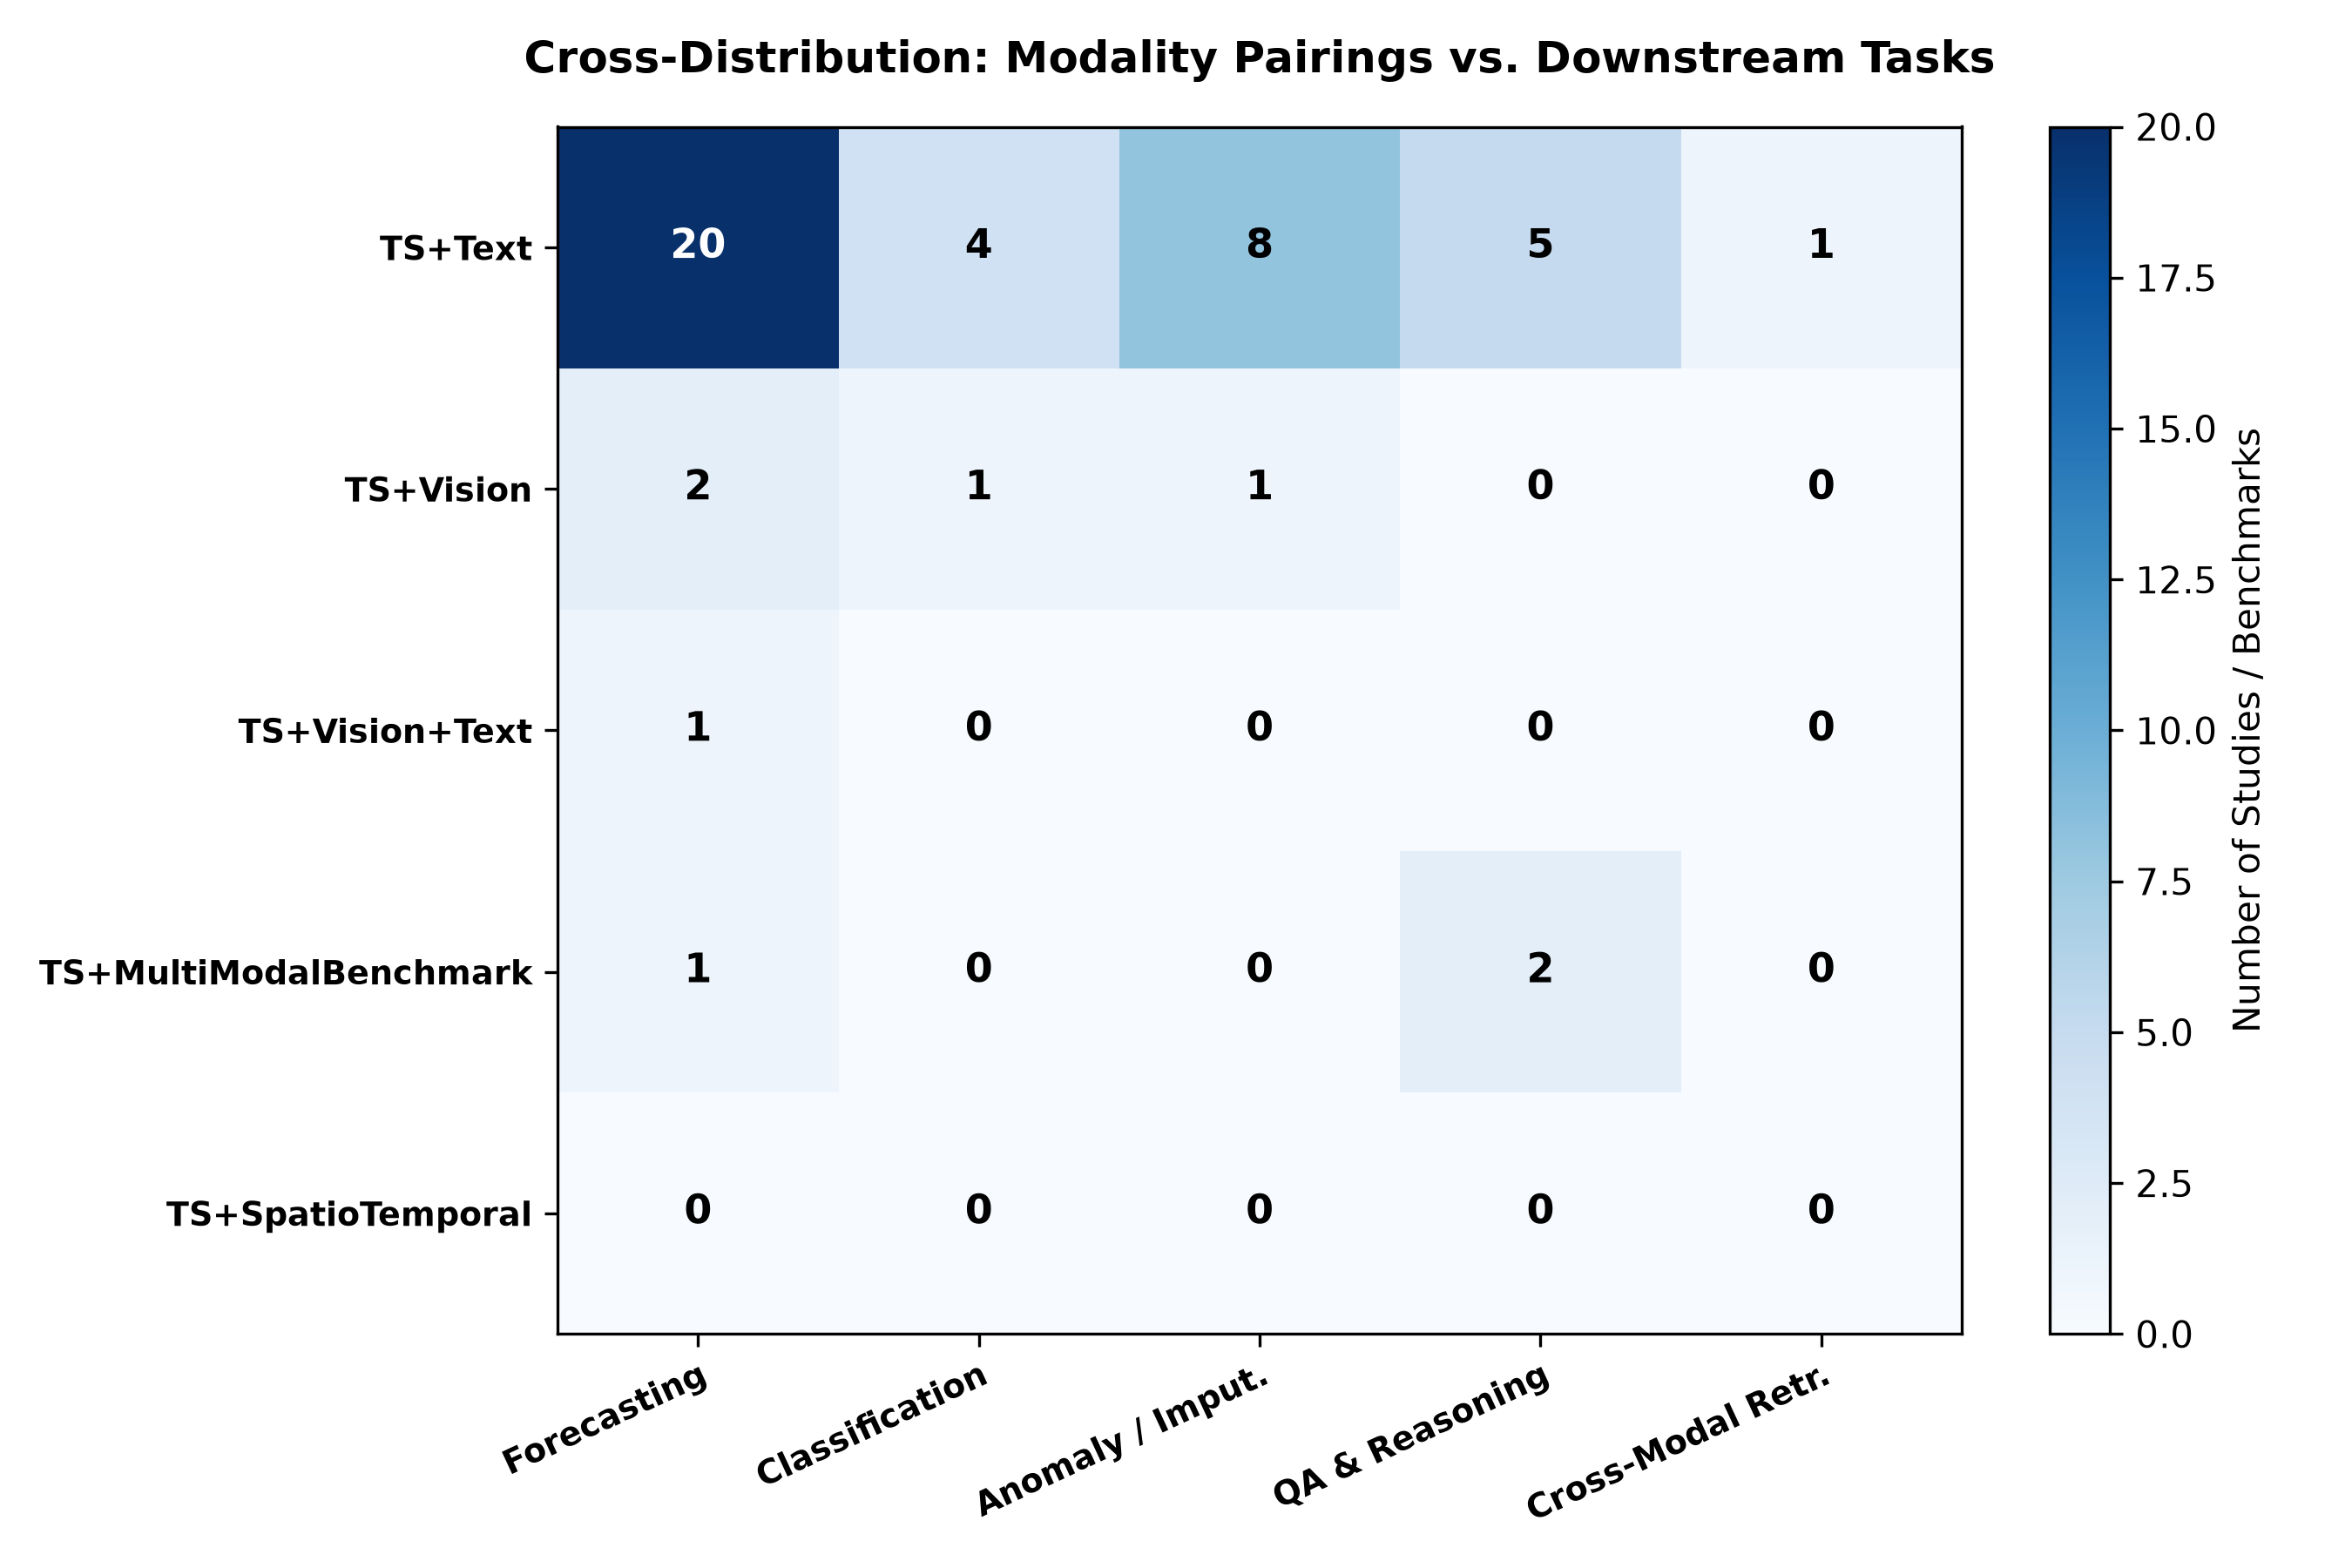
\includegraphics[width=0.48\textwidth]{figures/modality_task_heatmap.png}
\caption{Cross-distribution heatmap illustrating the frequency of studies evaluated across specific modality pairs and downstream predictive/reasoning tasks.}
\label{fig:heatmap}
\end{figure}

\begin{figure}[t]
\centering
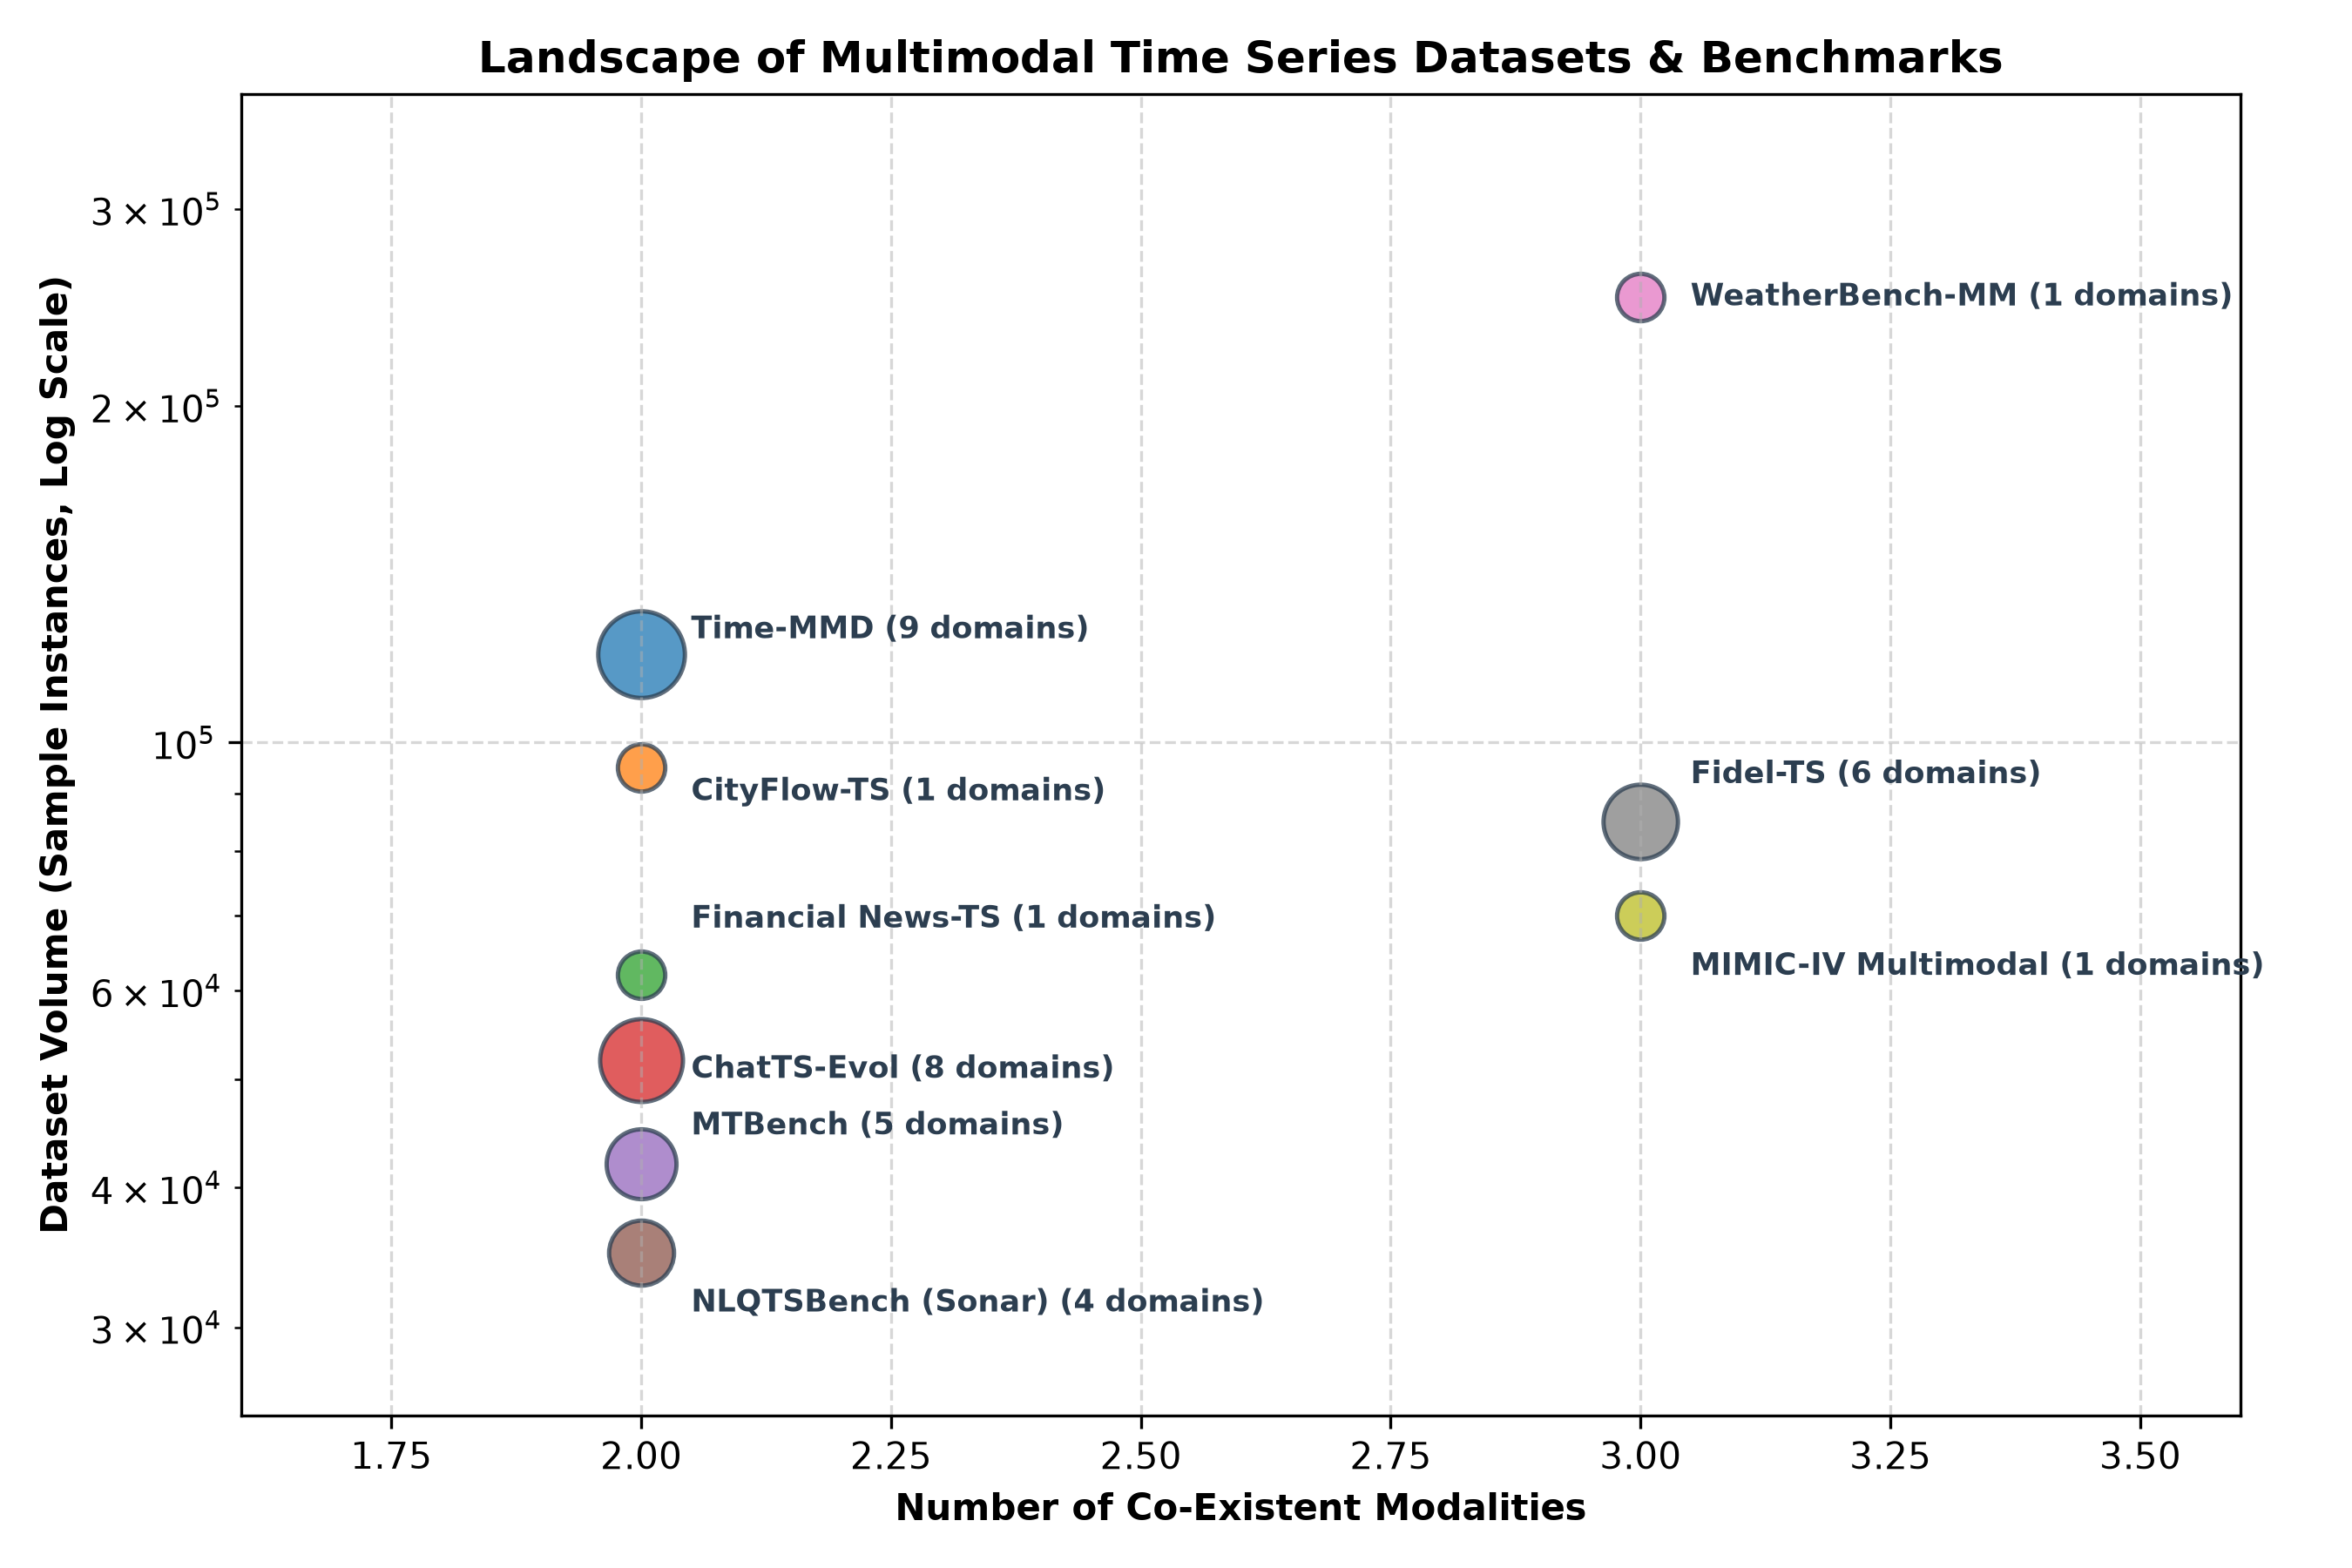
\includegraphics[width=0.48\textwidth]{figures/dataset_landscape.png}
\caption{Landscape of representative multimodal time-series datasets and benchmarks, comparing dataset sample instance volume (log scale) against the number of co-existent modalities.}
\label{fig:dataset_landscape}
\end{figure}

\subsection{Benchmark Suites and Multimodal Corpora}
As illustrated in \Cref{fig:dataset_landscape}, early multimodal experiments relied on ad-hoc combinations of univariate benchmark series (e.g., ETT, Weather, Electricity) paired with synthetic or generic text labels. Recently, comprehensive multi-domain suites have emerged:
\begin{itemize}
    \item \textbf{Time-MMD~\cite{Liu2024TimeMMD}:} Spanning 9 diverse domains (finance, energy, weather, healthcare, traffic, environment, agriculture, economy, and social media), Time-MMD provides fine-grained, timestamp-aligned textual context (e.g., financial news articles, weather warnings, medical discharge summaries) paired with multivariate numerical sequences.
    \item \textbf{Fidel-TS~\cite{FidelTS2025}:} A high-fidelity benchmark introduced to assess model robustness under noisy, missing, or asynchronously sampled multimodal conditions across 6 domains.
    \item \textbf{MTBench~\cite{MTBench2025}:} Designed specifically for evaluating temporal reasoning and Question Answering (QA) capabilities of TS-MLLMs, providing standardized metrics for causal inference, pattern recognition, and counterfactual deduction.
\end{itemize}

\begin{table}[t]
\caption{Overview of Prominent Multimodal Time-Series Datasets and Benchmarks.}
\label{tab:datasets}
\centering
\small
\setlength{\tabcolsep}{3pt}
\resizebox{\columnwidth}{!}{%
\begin{tabular}{llccc}
\toprule
\textbf{Dataset / Suite} & \textbf{Primary Domain} & \textbf{Modalities} & \textbf{Sample Volume} & \textbf{Target Tasks} \\
\midrule
Time-MMD~\cite{Liu2024TimeMMD} & 9 Diverse Domains & TS + Text & $\approx 1.2 \times 10^5$ & Forecasting \\
Fidel-TS~\cite{FidelTS2025} & Multi-Domain (6) & TS + Text + Vis & $\approx 8.5 \times 10^4$ & Robust Forecasting \\
MTBench~\cite{MTBench2025} & Multi-Domain (5) & TS + Text & $\approx 4.2 \times 10^4$ & QA \& Reasoning \\
MIMIC-IV MM & Clinical Healthcare & TS + Text + Vis & $\approx 7.0 \times 10^4$ & Mortality / Diag. \\
WeatherBench-MM & Meteorology & TS + Text + Vis & $\approx 2.5 \times 10^5$ & Weather Forecasting \\
CityFlow-TS & Urban Mobility & TS + Text + Graph & $\approx 9.5 \times 10^4$ & Traffic Forecasting \\
\bottomrule
\end{tabular}%
}
\end{table}

\begin{table*}[t]
\caption{Empirical Benchmark Meta-Table: Cross-Modal Model Performance across Representative Benchmarks. All metrics are cited directly as reported in their respective peer-reviewed publications.}
\label{tab:empirical_meta}
\centering
\scriptsize
\setlength{\tabcolsep}{3.5pt}
\resizebox{\textwidth}{!}{%
\begin{tabular}{llcccccccc}
\toprule
\multicolumn{10}{c}{\textbf{Panel A: Standard Long-Term Forecasting Benchmarks (Lookback $L=512$, Horizon $H=96$, Metric: MSE / MAE)}} \\
\midrule
\textbf{Model} & \textbf{Modality / Paradigm} & \multicolumn{2}{c}{\textbf{ETTh1}} & \multicolumn{2}{c}{\textbf{ETTm1}} & \multicolumn{2}{c}{\textbf{Weather}} & \multicolumn{2}{c}{\textbf{Electricity}} \\
& & MSE & MAE & MSE & MAE & MSE & MAE & MSE & MAE \\
\midrule
DLinear~\cite{Zhou2023OneFitsAll} & Unimodal Linear Baseline & 0.422 & 0.439 & 0.357 & 0.395 & 0.248 & 0.301 & 0.166 & 0.276 \\
PatchTST~\cite{Zhou2023OneFitsAll} & Unimodal Supervised Transformer & 0.413 & 0.435 & 0.351 & 0.389 & 0.225 & 0.270 & 0.161 & 0.264 \\
GPT4TS (One Fits All)~\cite{Zhou2023OneFitsAll} & TS + Text (Frozen GPT-2 Reprogram.) & 0.465 & 0.457 & 0.388 & 0.406 & 0.237 & 0.279 & 0.167 & 0.268 \\
Time-LLM~\cite{Jin2023TimeLLM} & TS + Text (LLaMA-7B Reprogram. + Prompts) & 0.408 & 0.428 & 0.329 & 0.364 & 0.225 & 0.264 & 0.158 & 0.258 \\
VisionTS (Zero-Shot)~\cite{Chen2024VisionTS} & TS + Vision (ImageNet ViT-Base MAE) & 0.381 & 0.406 & 0.334 & 0.370 & 0.174 & 0.219 & 0.148 & 0.247 \\
VisionTS (Full-Shot)~\cite{Chen2024VisionTS} & TS + Vision (Fine-tuned Visual MAE) & \textbf{0.347} & \textbf{0.382} & \textbf{0.281} & \textbf{0.339} & \textbf{0.142} & \textbf{0.191} & \textbf{0.126} & \textbf{0.228} \\
\midrule
\multicolumn{10}{c}{\textbf{Panel B: Time-MMD Aligned Multimodal Benchmark (Lookback $L=336$, Horizons $H \in \{48, 96, 192, 336\}$, Metric: MSE)}} \\
\midrule
\textbf{Domain / Dataset} & \textbf{Configuration} & \textbf{H=48} & \textbf{H=96} & \textbf{H=192} & \textbf{H=336} & \textbf{Average} & \multicolumn{3}{c}{\textbf{Multimodal Gain / Notes}} \\
\midrule
\multirow{4}{*}{Energy (Time-MMD)~\cite{Liu2024TimeMMD}} & DLinear & 0.24 & 0.33 & 0.38 & 0.52 & 0.368 & \multicolumn{3}{l}{Unimodal baseline} \\
& PatchTST & 0.20 & 0.30 & 0.34 & 0.48 & 0.330 & \multicolumn{3}{l}{Unimodal Transformer} \\
& Time-LLM (Unimodal, TS only) & 0.16 & 0.27 & 0.31 & 0.45 & 0.298 & \multicolumn{3}{l}{Ablation without text} \\
& Time-LLM (Multimodal, TS + Text) & \textbf{0.10} & \textbf{0.20} & \textbf{0.29} & \textbf{0.41} & \textbf{0.250} & \multicolumn{3}{l}{\textbf{$-16.1\%$ avg MSE ($-37.5\%$ at $H=48$)}} \\
\midrule
\multirow{4}{*}{Traffic (Time-MMD)~\cite{Liu2024TimeMMD}} & DLinear & 0.25 & 0.25 & 0.26 & 0.31 & 0.268 & \multicolumn{3}{l}{Unimodal baseline} \\
& PatchTST & 0.22 & 0.22 & 0.22 & 0.28 & 0.235 & \multicolumn{3}{l}{Unimodal Transformer} \\
& Time-LLM (Unimodal, TS only) & 0.21 & 0.21 & 0.21 & 0.27 & 0.225 & \multicolumn{3}{l}{Ablation without text} \\
& Time-LLM (Multimodal, TS + Text) & \textbf{0.19} & \textbf{0.20} & \textbf{0.20} & \textbf{0.27} & \textbf{0.215} & \multicolumn{3}{l}{\textbf{$-4.4\%$ avg MSE ($-9.5\%$ at $H=48$)}} \\
\midrule
\multicolumn{10}{c}{\textbf{Panel C: Planetary Earth System Forecasting on WeatherBench (Metric: Z500 Geopotential Height RMSE [$\text{m}^2/\text{s}^2$])}} \\
\midrule
\textbf{Model} & \textbf{Architecture Type} & \textbf{Lead 6h} & \textbf{Lead 24h} & \textbf{Lead 72h} & \textbf{Lead 120h} & \textbf{Lead 168h} & \multicolumn{3}{c}{\textbf{Operational Characteristics}} \\
\midrule
ClimaX~\cite{Nguyen2023ClimaX} & Variable-Tokenized Transformer & 62.73 & 96.19 & 244.08 & 440.40 & 599.43 & \multicolumn{3}{l}{Flexible variable subset pre-training} \\
FourCastNet~\cite{Nguyen2023ClimaX} & Fourier Neural Operator & 37.52 & 81.31 & 251.96 & 483.44 & 680.00 & \multicolumn{3}{l}{Fixed resolution and variable grid} \\
GraphCast~\cite{Nguyen2023ClimaX} & Spatial Graph Neural Network & 16.46 & 38.77 & 125.78 & 271.65 & 466.53 & \multicolumn{3}{l}{Specialized mesh message passing} \\
\midrule
\multicolumn{10}{c}{\textbf{Panel D: Specialized Modality Pairs: Clinical Healthcare and Acoustic Reprogramming}} \\
\midrule
\textbf{Task / Benchmark} & \textbf{Model} & \textbf{Modality Configuration} & \multicolumn{3}{c}{\textbf{Primary Metric}} & \multicolumn{4}{c}{\textbf{Key Empirical Finding}} \\
\midrule
\multirow{3}{*}{\shortstack[l]{Clinical ICU Prognosis\\(PhysioNet / MIMIC-IV)~\cite{Hayat2022MedFuse}}} & Unimodal LSTM & TS vitals only & \multicolumn{3}{c}{AUROC: $0.817$} & \multicolumn{4}{l}{Baseline clinical sequential modeling} \\
& Unimodal ResNet-34 & CXR image scans only & \multicolumn{3}{c}{AUROC: $0.803$} & \multicolumn{4}{l}{Static radiological image classification} \\
& MedFuse & TS vitals + CXR scans & \multicolumn{3}{c}{\textbf{AUROC: 0.874} ($95\%$ CI: $[0.860, 0.888]$)} & \multicolumn{4}{l}{\textbf{$+5.7\%$ AUROC over best unimodal baseline}} \\
\midrule
\multirow{2}{*}{\shortstack[l]{Acoustic Reprogramming\\(UCR 30-dataset suite)~\cite{Yang2021Voice2Series}}} & Baseline SOTA & Unimodal 1D deep nets & \multicolumn{3}{c}{Mean Acc: $\approx 83.2\%$} & \multicolumn{4}{l}{Standard supervised 1D TS architectures} \\
& Voice2Series & TS + Pretrained Acoustic Net & \multicolumn{3}{c}{\textbf{Mean Acc: 87.36\%}} & \multicolumn{4}{l}{\textbf{Outperforms unimodal SOTA on 19/30 datasets}} \\
\bottomrule
\end{tabular}%
}
\end{table*}

\subsection{Cross-Task Distribution Analysis}
\Cref{fig:heatmap} cross-tabulates the distribution of published works across modality combinations and downstream tasks. Several critical patterns emerge:
\begin{enumerate}
    \item \textbf{Dominance of Text-Guided Forecasting:} The overwhelming majority of contemporary studies focus on $\text{TS} + \text{Text}$ for forecasting ($n=20$), reflecting the direct applicability of pre-trained language models to temporal regression.
    \item \textbf{Emerging Frontier in QA and Reasoning:} While forecasting has reached high maturity, interactive QA, semantic reasoning, and explainable anomaly detection ($n=5$) represent the fastest-growing frontier.
    \item \textbf{Under-Explored Cross-Modal Retrieval:} Despite its industrial utility for database search, cross-modal retrieval ($\text{TS} \leftrightarrow \text{Text}$) remains nascent ($n=1$, pioneered by TRACE~\cite{Chen2025TRACE}).
\end{enumerate}

\subsection{In-Depth Empirical Analysis \& Findings}
Synthesizing the validated empirical numbers across the four panels of \Cref{tab:empirical_meta} reveals several fundamental insights into multimodal time-series learning:

\subsubsection{1. Visual Geometry vs.\ Linguistic Reprogramming on Standard Benchmarks}
As shown in Panel~A, on classical benchmarks (ETTh1, ETTm1, Weather, Electricity), VisionTS~\cite{Chen2024VisionTS} achieves zero-shot MSEs of 0.381 on ETTh1 and 0.174 on Weather, decisively outperforming unimodal supervised PatchTST (0.413 and 0.225) and GPT-2 reprogramming (GPT4TS, 0.465 and 0.237) without fine-tuning on a single time series point. When fully fine-tuned, VisionTS drops ETTh1 MSE to 0.347 and Weather MSE to 0.142. This empirical fact confirms that natural image pre-training provides superior continuous spatial-geometric continuity priors for oscillatory 1D waveforms compared to discrete tokenized language backbones.

\subsubsection{2. When Does Text Modality Provide Decisive Gains?}
Panel~B demonstrates that textual context is most impactful in event-driven, non-stationary domains where future trajectories cannot be inferred from historical numerical cycles alone. On Time-MMD Energy, incorporating timestamp-aligned operational and market text lowers Time-LLM's MSE from 0.16 to 0.10 at horizon $H=48$ (a 37.5\% error reduction) and maintains a 16.1\% overall reduction across all horizons. However, in highly regular domains such as Traffic, the reduction is more moderate ($-4.4\%$ overall), corroborating the auditing findings of Wang et al.~\cite{Wang2026AuditingText} that text provides diminishing returns when numerical periodicity already dominates the signal.

\subsubsection{3. Multi-Variable Scaling in Earth Systems}
Panel~C highlights the trade-offs of foundation models in physical systems. While specialized spatial graph architectures (GraphCast) achieve superior short-range accuracy through bespoke mesh geometry, ClimaX~\cite{Nguyen2023ClimaX} demonstrates remarkable multi-variable stability at extended lead times (RMSE 599.43 at 168 hours vs.\ 680.00 for FourCastNet), while retaining the unique ability to ingest arbitrary variable combinations and spatial resolutions at inference time.

\subsubsection{4. Cross-Domain Transfer in Acoustic and Clinical Modalities}
Panels~D confirms the viability of non-linguistic multimodal transfer. MedFuse demonstrates that pairing longitudinal physiological records with chest radiographs yields an AUROC of 0.874 for ICU in-hospital mortality prediction, representing a 5.7\% absolute gain over unimodal LSTM sequence models. Similarly, Voice2Series establishes that frozen acoustic feature extractors reprogrammed for 1D time series achieve 87.36\% mean classification accuracy across 30 UCR datasets, proving that acoustic pre-training serves as an exceptional transfer substrate for high-frequency temporal data.

\section{Open Challenges and Future Trajectories}
\label{sec:outlook}

Despite rapid progress, multimodal time series intelligence faces foundational theoretical and engineering hurdles. In this section, we delineate five open challenges and outline promising future research directions.

\subsection{1. The Continuous-to-Discrete Modality Gap}
While natural language and visual objects exhibit discrete, hierarchical compositional semantics, physical time series are continuous, non-stationary, and governed by fine-grained numerical gradients. Discretizing numerical time series into discrete vocabulary tokens (e.g., via scalar binning or k-means codebooks) often results in loss of numerical precision or boundary artifacts. Conversely, continuous patch projections frequently suffer from representational collapse when aligned with high-dimensional language embeddings. Developing principled cross-modal mapping functions that preserve continuous physical conservation laws while tapping into discrete semantic reasoning remains an unresolved challenge.

\subsection{2. Asynchronous Sampling and Irregular Multimodal Streams}
In real-world operational environments, data modalities arrive at vastly different temporal granularities. For instance, high-frequency IoT sensor telemetry is collected millisecond-by-millisecond, financial market prices tick second-by-second, news reports appear intermittently, and satellite passes occur weekly. Current models predominantly rely on artificial resynchronization (e.g., forward filling or downsampling), which discards high-frequency signal content or introduces artificial latency. Future architectures must incorporate continuous-time neural ordinary differential equations (Neural ODEs) or state-space models (SSMs) to natively handle asynchronous, irregularly sampled multimodal streams.

\subsection{3. Evaluation Integrity: Benchmark Contamination and Data Leakage}
A persistent concern in the evaluation of LLM-adapted time series forecasters is the risk of training data contamination. Pre-trained web-scale language models (e.g., GPT-4, LLaMA) have ingested massive portions of GitHub repositories, academic papers, and publicly hosted datasets (such as the standard ETT, Weather, and Electricity benchmarks). Consequently, models claiming "zero-shot" forecasting prowess may in fact be performing memorized retrieval of benchmark statistical properties. Establishing contamination-resistant benchmarks, strictly partitioned temporal splits, and dynamic online evaluation protocols is imperative for scientific credibility.

\subsection{4. Computational Latency and Edge Deployment Bottlenecks}
Modern foundation LLMs and VLMs span billions of parameters (7B to 70B), demanding extensive GPU memory and incurring inference latencies measured in hundreds of milliseconds. In contrast, mission-critical time series applications—such as electrical grid fault isolation, surgical patient monitoring, and autonomous vehicle control—mandate sub-10-millisecond response times. Parameter-efficient distillation, specialized lightweight time-series mixers (such as Tiny Time Mixers~\cite{Ekambaram2024TTM}), and edge-optimized hardware accelerators represent crucial avenues for practical industrial adoption.

\subsection{5. Neuro-Symbolic Agentic Frameworks and Database NLQ}
Looking forward, the frontier of multimodal time series is shifting from passive predictive models toward active, autonomous analytical agents. As demonstrated by recent neuro-symbolic querying frameworks, future systems will seamlessly couple LLM reasoning controllers with formal database query execution engines (e.g., SQL and vector indexing over time-series databases). These agents will formulate hypotheses, write verification code, interrogate terabyte-scale sensor repositories via natural language, and deliver auditable, explainable insights to domain experts.

\section{Conclusion}
\label{sec:conclusion}
This survey has presented the first systematic, PRISMA 2020-compliant review of Multimodal Time Series Models from 2021 to 2026. By proposing a unified multi-dimensional taxonomy, providing deep mathematical dissections of cross-modal reprogramming, visual rendering, and conversational reasoning architectures, and mapping the evolving dataset landscape, we establish a structured foundation for this rapidly expanding field. As multimodal foundation models continue to bridge the divide between continuous physical observations and discrete human reasoning, multimodal time series intelligence promises to redefine scientific discovery, industrial automation, and healthcare monitoring.


\bibliographystyle{IEEEtran}
\bibliography{references}

\end{document}
